\chapter{Introduzione}

Il riconoscimento dell'attività umana (Human Activity Recognition, HAR) è un campo molto attivo della ricerca e una
quantità sempre maggiore di tecniche di \textit{deep learning} sviluppate negli ultimi anni ha dimostrato di essere 
affidabile per la classificazione delle attività di vita quotidiana (Activities of Daily Living, ADLs).

Un aspetto che lega la quasi totalità delle tecniche messe in campo quando si parla di HAR è sicuramente l'ottenimento delle informazioni 
utili per le analisi. Per il riconoscimento di una attività sono indubbiamente necessari i dati ottenuti dai
sensori di movimento posizionati sui nostri smartphone o sui sempre più comuni braccialetti ed orologi intelligenti.

\section{Classificazione}
Il riconoscimento delle attività si basa sulla \textit{classificazione}, un problema statistico che ha l'obiettivo di ipotizzare 
quale tra un insieme di etichette meglio definisce un insieme di caratteristiche. 

La classificazione, in informatica, è un ramo dell'apprendimento supervisionato (\textit{supervised learning}),
ovvero una branca dell'apprendimento automatico (\textit{machine learning}) che punta ad insegnare ad un sistema informatico una regola generale
di calcolo su un certo dominio di dati in modo che successivamente sia in grado di applicare in autonomia le stesse leggi anche a dati futuri.

Definiamo quindi \textbf{classificatore} un algoritmo in grado di risolvere il problema della classificazione, in grado di fornire in output 
l'etichetta che meglio identifica i dati ricevuti in input.
Nel caso in esame il classificatore dovrà essere in grado di ipotizzare una attività ricevendo in input un set di dati sensoriali
raccolti dall'applicazione sviluppata.

\subsection{L'importanza dei dati}
Ipotizzando che la qualità dei dati sia ottima (o almeno sufficiente), l'aspetto di cui bisogna assolutamente tener conto quando 
si parla di apprendimento automatico è la quantità di dati che si è in grado di raccogliere. 
L'efficienza e l'efficacia di un classificatore, in generale, si basano interamente sui valori precedentemente appresi.

La necessità di un set di dati ampio per l'apprendimento è principalmente conseguenza del fatto che non viviamo in un mondo ideale: 
le attività svolte nella vita reale non sono perfettamente suddivisibili per essere facilmente classificate e inoltre, dato che diverse persone
potrebbero svolgere una uguale attività in modi differenti, non si ha nemmeno una corrispondenza biunivoca tra un insieme di dati e l'attività \cite{framework_long_term_data_har}.

\subsubsection{Dati necessari per il riconoscimento}
È già stato anticipato che i dati su cui solitamente si basa lo sviluppo di un classificatore per il riconoscimento di una attività sono forniti dai 
più comuni sensori di movimento.

Ad essi ne possono essere aggiunti di ulteriori, come ad esempio le informazioni sulle caratteristiche fisiche
dell'individuo o sulla posizione in cui è situato il dispositivo di raccolta.

\section{Obiettivo e panoramica del progetto}
Lo scopo del progetto è quindi lo sviluppo di un classificatore di ADLs in grado di interagire con una applicazione
Android.

\begin{figure}[H]
    \centering
    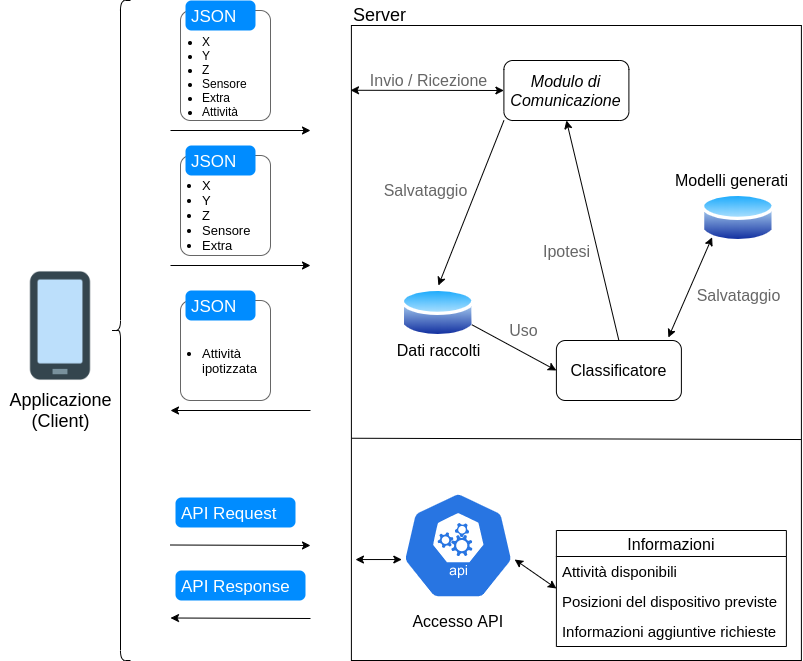
\includegraphics[scale = 0.41]{assets/images/overview.png}
    \caption{Panoramica del progetto}
    \label{fig:overview}
\end{figure}

\subsubsection{Applicazione}
L'applicazione Android ha il compito di ottenere i dati relativi ai movimenti dell'utente 
e gestire lo scambio di tutte le informazioni raccolte con il server.
\subsubsection{Classificatore}
Il componente che effettuerà la classificazione, che come abbiamo detto, gestirà la mole di valori ottenuta tentando di 
eseguire il riconoscimento vero e proprio delle attività.
\subsubsection{Rest API}
Sono poi state aggiunte delle API Rest utilizzate come fonte iniziale di informazioni. Vedremo essere indispensabili 
per rendere l'intero sistema programmabile in modo dinamico, almeno per quanto riguarda tutto ciò che sarà impostabile 
da un amministratore in fase di avvio.